\chapter{Experimental setup}\label{chap:02}

The measurement system employs an Alibava EASy radiation detection platform comprising three primary components:
\begin{enumerate}
    \item \textbf{Detector unit}: Silicon microstrip sensor assembly
    \item \textbf{Control unit}: Signal processing and interface electronics
    \item \textbf{Data acquisition computer}: System control and analysis
\end{enumerate}

Interconnections between components are established through:
\begin{itemize}
    \item Ribbon cable (detector $\leftrightarrow$ control unit)
    \item USB interface (control unit $\leftrightarrow$ computer)
    \item Optional optical fiber for specialized measurements
\end{itemize}

System operation is managed through the Alibava Graphical User Interface (GUI), which provides:
\begin{itemize}
    \item Real-time detector control
    \item Measurement configuration
    \item Data visualization and acquisition
\end{itemize}

In some measuring tasks, an additional optical fiber cable is used. In the source measurements, a radioactive source ($^{90}\mathrm{Sr}$) and a LEMO cable for the built-in diode are needed.
%----------------------------------------------------%
\section{Detector unit}

The detector unit employs a semiconductor sensor integrated with dedicated readout electronics. Positioned above the sensor assembly, a configurable laser system provides controlled excitation for signal generation. This laser features two operational orientations: the \enquote{L} position facilitates laser-based calibration measurements, while the \enquote{Q} position enables radioactive source characterization. 

Signals generated within the sensor undergo amplification and processing through the BEETLE application-specific integrated circuit which converts charge pulses into digitizable voltage waveforms. The BEETLE chip incorporates a pipeline buffer that temporarily stores processed signals until receipt of an external trigger command from the control unit. Only triggered events are transmitted for further analysis; untriggered data streams are systematically discarded to optimize data throughput.

\begin{figure}[H]
       %\setkeys{Gin}{draft=false}
	\centering
	%\fcolorbox{black}{white}{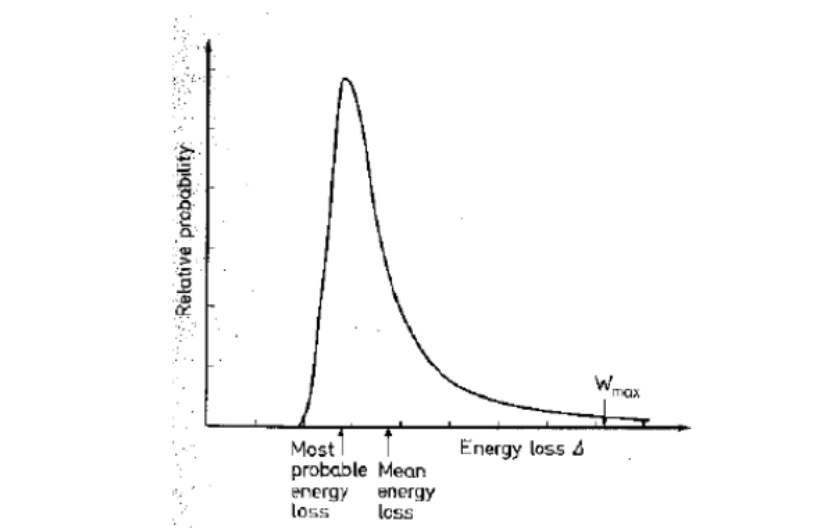
\includegraphics[scale=0.3]{pictures/landau.png}}
        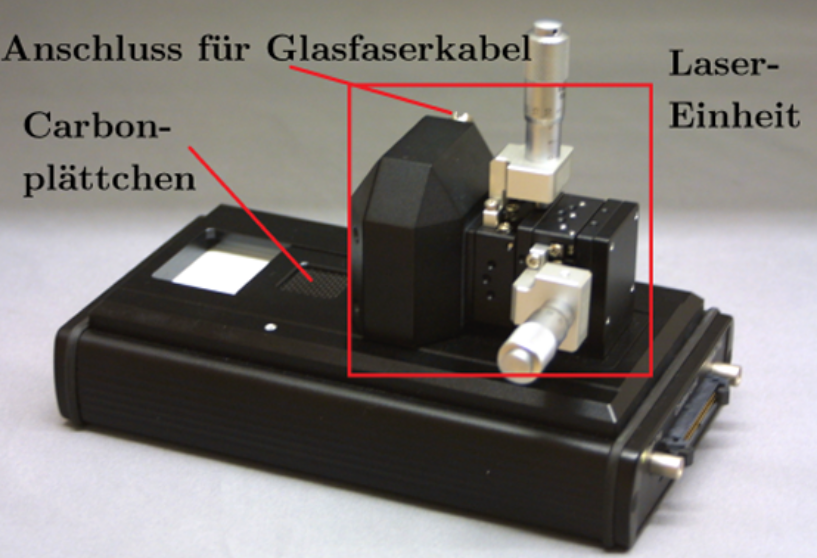
\includegraphics[width=0.41\textwidth]{pictures/detector1.png}
        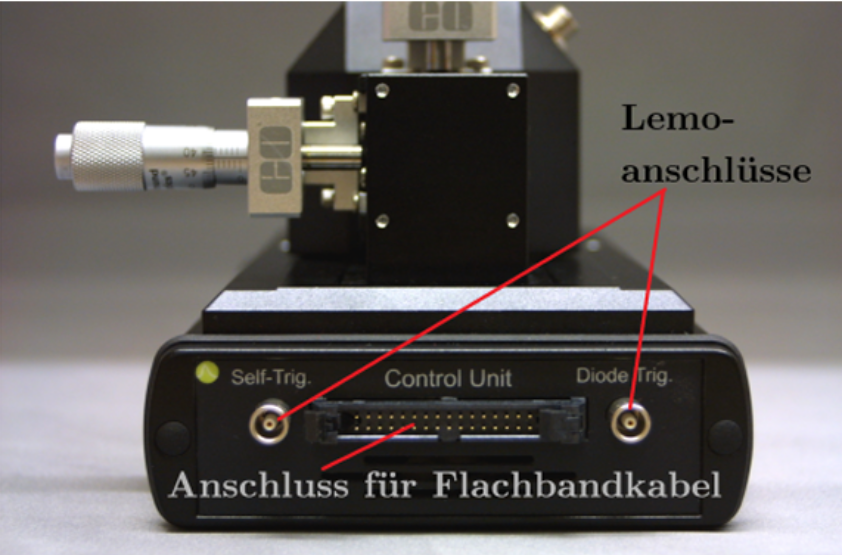
\includegraphics[width=0.43\textwidth]{pictures/detector2.png}
	\caption{The detector unit in \enquote{Q} position. Top view (left) and side view (right).}
        \label{fig:detector1}   
\end{figure}

The detection element consists of a 300 $\mu$m thick n-doped silicon substrate. One surface features a continuous metallization layer, while the opposite face contains 128 electrically isolated p-doped strip implants. This configuration establishes a p-n junction architecture, specifically categorized as a p-in-n sensor due to the p-type implants embedded within the n-type bulk material. Electrical isolation between adjacent strips prevents inter-strip conduction, enabling spatial resolution of incident radiation through channel-specific signal readout. A silicon oxide layer suppresses surface leakage currents that could compromise signal integrity.

The sensor incorporates two critical peripheral structures: a guard ring that confines charge carriers within the active detection area, and a bias ring that applies the operational voltage to establish the depletion zone. \autoref{fig:detector1} illustrates the detector unit in the "Q" configuration, while \autoref{fig:detector2} provides detailed schematics of the sensor geometry.

Application of reverse bias voltage ($U_{\mathrm{bias}}$) generates an internal electric field that separates electron-hole pairs created by ionizing events. Below the depletion threshold, significant carrier recombination occurs in undepleted regions, degrading signal amplitude. The charge collection efficiency (CCE) quantifies this behaviour according to:

\begin{equation}
    \mathrm{CCE}(U) = \frac{1 - \exp\left(-\dfrac{d_c(U)}{a}\right)}{1 - \exp\left(-\dfrac{D}{a}\right)} \label{eq:fitdepl}
\end{equation}
where $D = 300\ \mu\mathrm{m}$ is the sensor thickness, $d_c(U)$ represents the voltage-dependent depletion depth, and $a$ denotes the mean laser penetration depth in silicon. CCE increases monotonically with applied voltage until reaching full depletion at $U_{\mathrm{dep}} \approx 60-70\ \mathrm{V}$, beyond which it plateaus at maximum efficiency. For electron excitation measurements, signal amplitude scales directly with $d_c(U)$.

\begin{figure}[H]
       %\setkeys{Gin}{draft=false}
	\centering
	%\fcolorbox{black}{white}{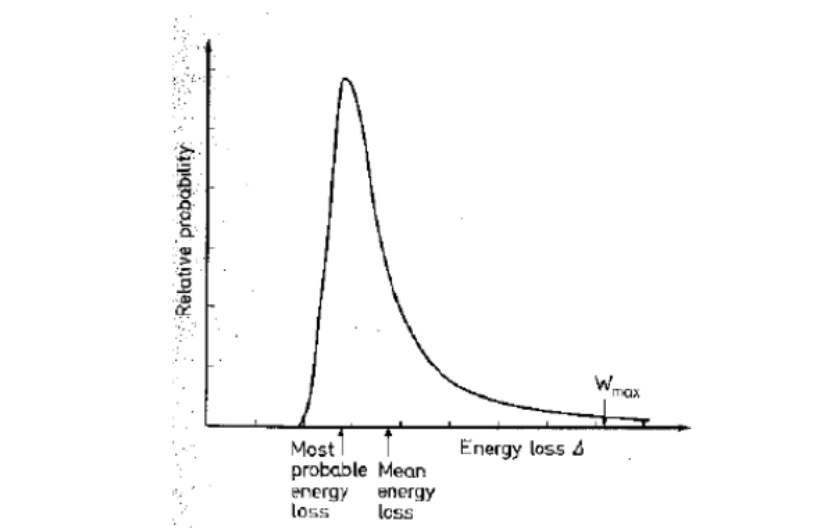
\includegraphics[scale=0.3]{pictures/landau.png}}
        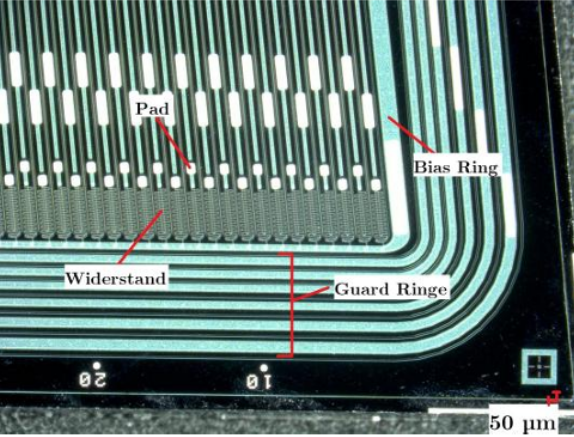
\includegraphics[width=0.43\textwidth]{pictures/detector3.png}
        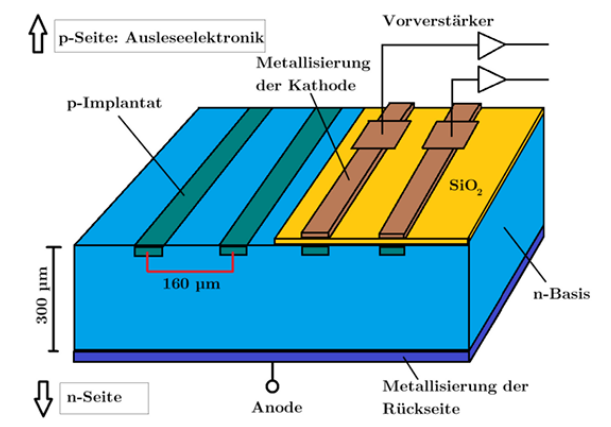
\includegraphics[width=0.43\textwidth]{pictures/detector4.png}
	\caption{Macroscopic top down view (left) and a schematic view of the construction of the whole sensor (right).}
        \label{fig:detector2}   
\end{figure}
%----------------------------------------------------%
\section{Laser}

The experimental setup incorporates a dedicated laser system for detector calibration. This laser source operates at 980 nm wavelength and delivers optical pulses to the detector unit through a fiber-optic interface. Key beam parameters include a 20 $\mu$m spot diameter, 5 ns pulse duration, and 0.2 mW peak optical power.

Precise spatial control of the laser illumination is achieved via a dual-axis micrometer screw assembly, enabling accurate positioning and focal adjustment on the sensor surface. This calibration subsystem provides controlled localized excitation for characterizing detector response and spatial resolution.
%----------------------------------------------------%
\section{Control unit}

The control unit serves as the central interface for detector operation, providing three primary functions: laser illumination control, sensor bias voltage regulation, and signal acquisition. This unit processes raw detector outputs into digital ADC counts that are subsequently recorded by the data acquisition computer. Additionally, it incorporates an amperometer capable of measuring leakage currents with a resolution of 0.01 $\mu$A.

To discriminate between noise and events detection, a statistical threshold is applied. For this experiment, signals must exceed the noise floor by at least five standard deviations ($5\sigma$) to be considered valid. Events failing this signal-to-noise criterion are excluded from further analysis.

Further signal integrity challenges arise from spatial effects within the strip detector geometry. When ionizing particles traverse near strip boundaries, induced charge may trigger multiple adjacent strips despite originating from a single physical event. This edge effect is compounded by crosstalk phenomena, where non-perpendicular particle trajectories deposit charge across several strips. Both effects necessitate sophisticated position reconstruction algorithms to correctly identify individual particle interactions.

The control unit's integrated measurement capabilities extend to continuous monitoring of sensor leakage currents. Processed ADC data streams are transmitted via USB to the acquisition computer, where the Alibava software platform enables data collection and system control.
%----------------------------------------------------%
